\chapter{Lavori correlati}
\label{ch:lavori-correlati}

\section{Contesto della Ricerca}
\label{sec:contesto-della-ricerca}
In questo capitolo verranno presentati alcuni lavori
correlati all'oggetto di questo lavoro.
In particolare saranno introdotti alcuni concetti chiave e
verranno discussi in modo da poter contestualizzare meglio
il lavoro svolto.

\section{LLM, modelli di linguaggio}
\label{sec:llm-modelli-di-linguaggio}
I Large Language Models (LLM) rappresentano una classe di
modelli di deep learning che hanno dimostrato capacità
straordinarie nel comprendere e generare testo in
linguaggio naturale.
Questi modelli sono addestrati su enormi quantità di dati
testuali e sono in grado di apprendere complesse relazioni
semantiche e sintattiche tra le parole.

Nel contesto del rilevamento di spoiler, gli LLM offrono un
potenziale significativo grazie alla loro capacità di
comprendere il contesto e il significato delle parole.
A differenza dei modelli basati su regole o su approcci di
machine learning tradizionali, gli LLM potrebbero catturare
sfumature semantiche e identificare spoiler anche in testi
complessi e ambigui.

I primi modelli di LLM utilizzavano una architettura del
tipo \textit{encoder-decoder} per generare testo in
linguaggio naturale.
L'encoder è responsabile di trasformare il testo in input
in una rappresentazione vettoriale, mentre il decoder è
responsabile di generare il testo in output.

Con l'introduzione del \textbf{meccanismo di attenzione}, i
modelli LLM sono diventati sempre più potenti e
sofisticati.
Il meccanismo di attenzione permette al modello di estrarre
il contesto delle parole nel testo, migliorando
notevolemente le performance in una varietà di task.

L'attenzione è stata successivamente estesa a modelli
\textit{attention-based}, come il Transformer.

\subsection{Attention is all you need}
\label{sec:attention-is-all-you-need}
Il Transformer è un modello di deep learning
\textit{attention-based} introdotto da Vaswani et al.
nel 2017 nel paper ``Attention is
all you need''\cite{vaswani2017attention}.
Il Transformer ha rivoluzionato il campo del deep learning
per il linguaggio naturale, superando i modelli
\textit{encoder-decoder} in termini di performance e
efficienza \cite{google2017transformer}.

Il meccanismo di attenzione è il cuore del Transformer.
Questo meccanismo permette al modello di assegnare pesi
diversi alle parole nel testo in input, in modo da poter
focalizzare l'attenzione sulle parole più rilevanti per il
testo in input.

\begin{figure}[H]
  \centering
  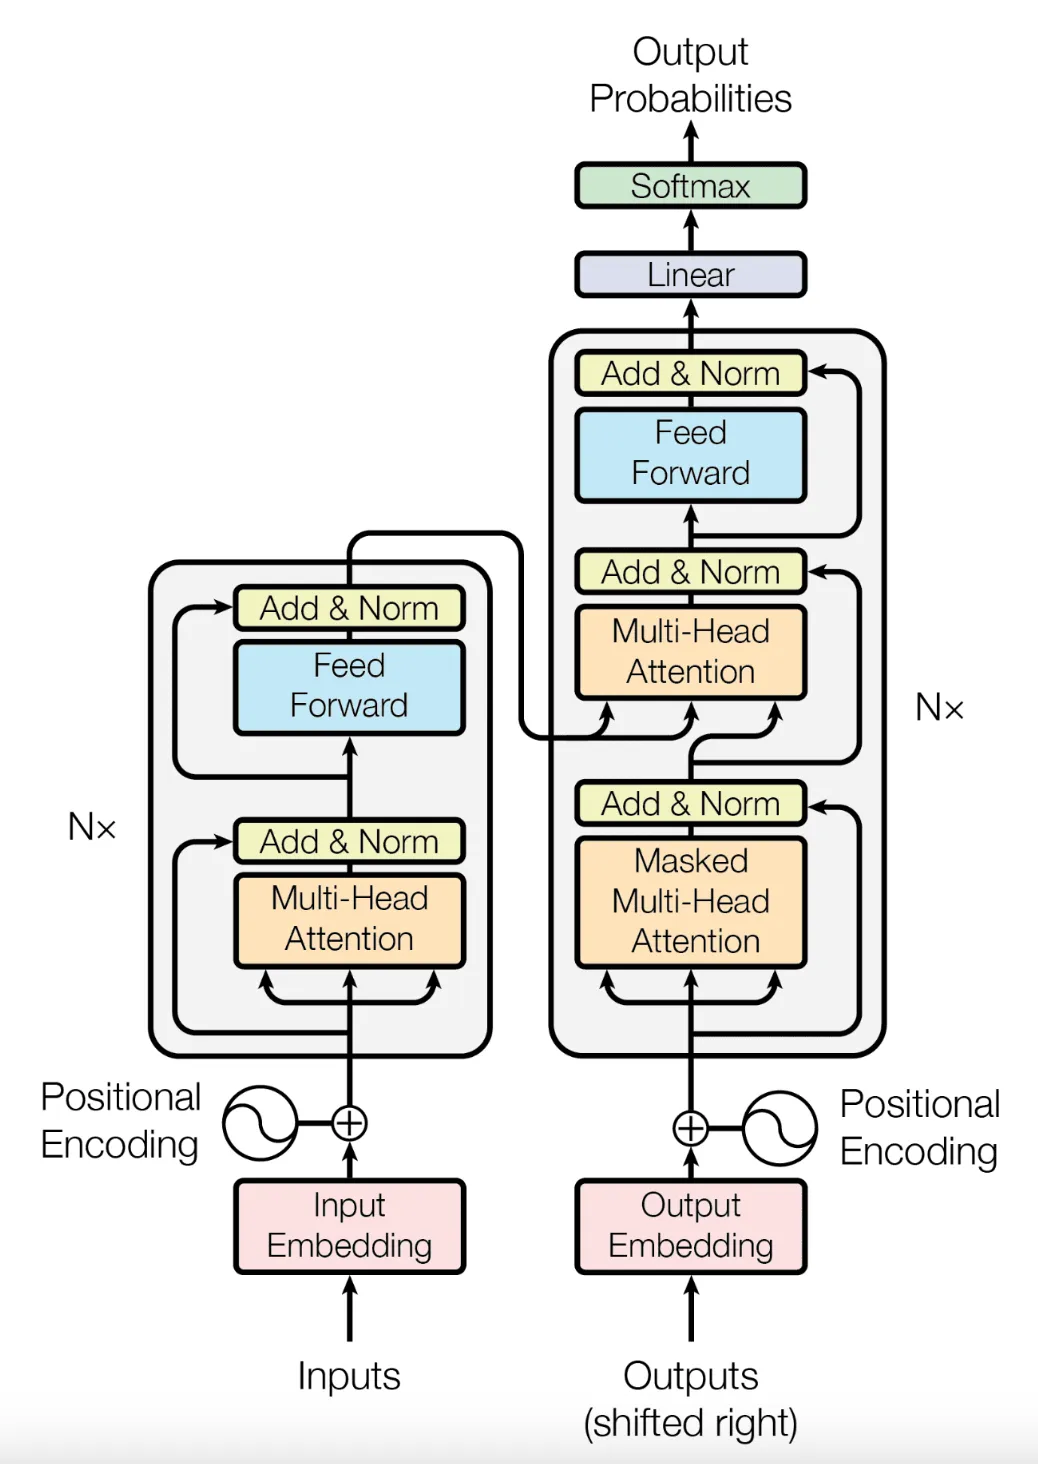
\includegraphics[width=0.6\textwidth]{res/transformer.png}
  \caption{Architettura del Transformer}
  \label{fig:transformer-architecture}
\end{figure}

\section{Embedding}
\label{sec:embedding}
Gli embedding sono una rappresentazione vettoriale di un
oggetto in uno spazio vettoriale.
Sono ampiamente utilizzati nel campo del deep learning per
rappresentare parole, frasi, documenti e immagini in modo
da poter essere usati come input per modelli di machine
learning \cite{mikolov2013efficient}.
Gli embedding vengono creati utilizzando modelli che
imparano a \textit{mappare} gli oggetti in uno spazio
vettoriale in modo che oggetti simili siano vicini tra
loro.
Tra i modelli di embedding più comuni troviamo
\textbf{Word2Vec}, \textbf{GloVe} e \textbf{FastText}.

Alcune delle applicazioni per gli embedding includono:

\begin{itemize}
  \item \textbf{Elaborazione del linguaggio naturale}: embedding
        di parole e frasi per modelli di classificazione,
        clustering e generazione di testo.
        Consentono al modello di comprendere il significato delle
        parole.
  \item \textbf{Sistemi di raccomandazione}: utilizzare gli
        embedding per rappresentare utenti, prodotti, post in uno
        spazio vettoriale, in modo da poterne calcolare la similarità.
  \item \textbf{Ricerca di immagini}: permettono di comparare
        immagini tra di loro o di comparare immagini e testo.
        Questo permette di cercare immagini tramite testo o
        viceversa.
  \item \textbf{Ricerca semantica}: rendono possibile la ricerca di
        frasi o documenti simili in base al loro significato.
\end{itemize}

Eseguire operazioni su embedding è molto più efficiente se
vengono memorizzati in un database apposito.

\begin{figure}[H]
  \centering
  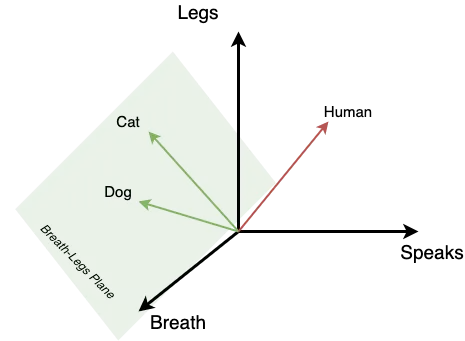
\includegraphics[width=0.5\textwidth]{res/embedding_space.png}
  \caption{Esempio di embedding. Fonte: \cite{olegborisovembeddingspace}}
  \label{fig:embedding-example}
\end{figure}

\subsection{Vector Database}
\label{sec:vector-database}
A differenza dei database tradizionali, i vector database
sono progettati per memorizzare e interrogare dati in forma
vettoriale.
Questo permette di effettuare operazioni e manipolazioni su
dati vettoriali in maniera più efficiente rispetto ad un
database relazionale.

I vector database sono particolarmente utili per
applicazioni che richiedono il calcolo della similarità tra
oggetti in uno spazio vettoriale, come le applicazioni
menzionate in precedenza.

Recentemente sono stati introdotti diversi vector database
come \textbf{Pinecone}, \textbf{Chroma} e \textbf{MongoDB
  Atlas}, ma per questo lavoro è stato scelto
\textbf{PostgreSQL} con il modulo \textit{PGVector} per
semplicità di utilizzo e familiarità.

\section{Fine-tuning di modelli}
\label{sec:finetuning-di-modelli}

Il finetuning è una tecnica comune nel campo del deep
learning per adattare un modello ad un task specifico.

Nel contesto del rilevamento di spoiler, il finetuning di
un modello può essere utile per migliorare le performance
del modello nel rilevare spoiler in un determinato contesto
o linguaggio.

Il finetuning di un modello pre addestrato comporta
l'addestramento del modello su un dataset specifico per un
numero limitato di epoche.
Questa tecnica consente di sfruttare le conoscenze
pregresse del modello, evitando di investire tempo e
risorse per addestrare un nuovo modello da zero.

Durante il finetuning, i pesi del modello vengono
aggiornati utilizzando un tasso di apprendimento più basso
rispetto all'addestramento iniziale.
Questo permette al modello di adattarsi al nuovo dataset
senza peggiorare le prestazioni su dati già visti.

Ciò risulta particolarmente utile quando si dispone di un
dataset limitato o quando si desidera adattare un modello
pre-addestrato a un dominio specifico.

\newpage
\section{Transizione all'implementazione}
\label{sec:transizione-implementazione}
Avendo stabilito il contesto teorico e tecnologico nel
capitolo corrente, il prossimo passo consiste nel
descrivere come questi concetti sono stati applicati nella
pratica.
Nel prossimo capitolo ci focalizzeremo sugli aspetti
pratici della realizzazione del sistema.
Descrivendo in dettaglio il design e l'implementazione del
sistema di rilevamento di spoiler, illustrando le sfide
incontrate e le soluzioni adottate per creare un sistema
efficace e utilizzabile.
